\documentclass{assignment}
\UsingEnglish
\ProjectInfos*{Intro to Communication System}{EE140}{Fall, 2020}{Assignment 4}{Due time : 10:15, Oct 16, 2020 (Friday)}{陈稼霖}{45875852}
\begin{document}
\begin{prob}[Different Analog Modulation Schemes, 20 pts]
    Using the massage signal $m(t)=10\cos 10\pi t$ and modulation carrier $C(t)=2\cos 200\pi t$, determined signals (time domain expression) for the following methods of modulation, and draw the spectrum of the modulation signals.
    \begin{itemize}
        \item[a)] Double-sideband-suppressed carrier (DSB-SC) modulation.
        \item[b)] Double-sideband, Large carrier (DSB-LC) modulation with modulation index $a=0.1$.
        \item[c)] Single-sideband (SSB) modulation with upper sideband retained.
        \item[d)] Vestigial-sideband (VSB) modulation with following VSB filter $H(f)$ in Figure 1.
    \end{itemize}
    \begin{figure}
        \centering
        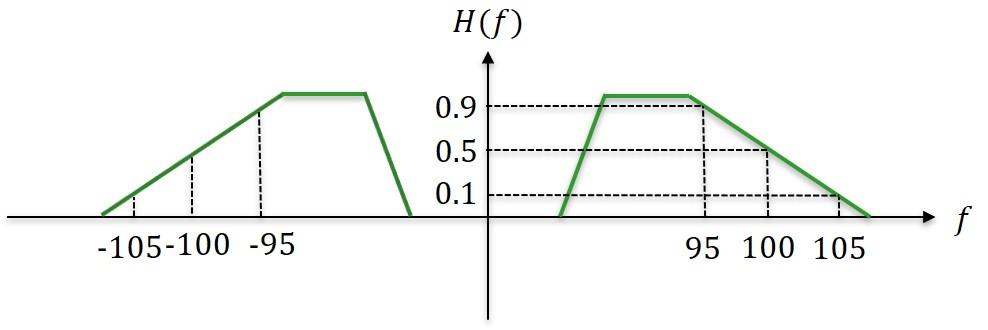
\includegraphics[width=.5\columnwidth]{Assignment-4-Problem-1.jpg}
        \caption{}
        \label{Assigment-4-Problem-1}
    \end{figure}
\end{prob}
\begin{sol}
    \begin{itemize}
        \item[a)] The modulated signal of DSB-SC modulation is
        \begin{align}
            x_c(t)=m(t)C(t)=20\cos(10\pi t)\cos(200\pi t)=20\cos(10\pi t)\cos(200\pi t)=10[\cos(190\pi t)+\cos(210\pi t)].
        \end{align}
        Its spectrum is
        \begin{align}
            X_c(f)=\mathscr{F}[x_c(t)]=5[\delta(f-95\pi)+\delta(f+95\pi)+\delta(f-105\pi)+\delta(f+105\pi)],
        \end{align}
        as shown in figure.
        \item[b)] The modulated signal of DSB-LC modulation with modulation index $a=0.1$ is
        \begin{align}
            \notag x_c(t)=&2\left[1+a\frac{m(t)}{\min[\abs{m(t)}]}\right]\cos(200\pi t)\\
            \notag=&2\left[1+0.1\frac{10\cos(10\pi t)}{10}\right]\cos(200\pi t)\\
            \notag=&2\cos(200\pi t)+0.2\cos(10\pi t)\cos(200\pi t)\\
            =&2\cos(200\pi t)+0.1[\cos(190\pi t)+\cos(210\pi t)].
        \end{align}
        Its spectrum is
        \begin{align}
            X_c(f)=\delta(f-100)+\delta(f+100)+0.05[\delta(f-95)+\delta(f+95)+\delta(f-105)+\delta(f+105)].
        \end{align}
        as shown in figure.
        \item[c)] The Hilbert transform of the message signal is
        \begin{align}
            \hat{x}(t)=10\sin(10\pi t).
        \end{align}
        The modulated signal of SSB modulation with upper sideband retained is
        \begin{align}
            \notag x_c(t)=&\frac{1}{2}2m(t)\cos(200\pi t)-\frac{1}{2}2\hat{m}(t)\sin(200\pi t)\\
            \notag=&10\cos(10\pi t)\cos(200\pi t)-10\sin(10\pi t)\sin(200\pi t)\\
            =&10\cos(210\pi t).
        \end{align}
        Its spectrum is
        \begin{align}
            X_c(f)=5[\delta(f-105)+\delta(f+105)],
        \end{align}
        as shown in figure.
        \item[d)] The spectrum of the message signal is
        \begin{align}
            M(f)=\mathscr{F}[m(t)]=5[\delta(f-5)+\delta(f+5)].
        \end{align}
        The spectrum of the signal of VSB modulation with VSB filter $H(f)$ is Figure \ref{Assigment-4-Problem-1} is
        \begin{align}
            \notag X_c(f)=&[M(f-100)+M(f+100)]H(f)\\
            \notag=&5[\delta(f-105)+\delta(f-95)+\delta(f+95)+\delta(f+105)]H(f)\\
            =&0.5\delta(f-105)+4.5\delta(f-95)+4.5\delta(f+95)+0.5\delta(f+105),
        \end{align}
        as shown in figure.
        The modulated signal of VSB is
        \begin{align}
            x_c(t)=\mathscr{F}^{-1}[X_c(f)]=9\cos(190\pi t)+\cos(210\pi t).
        \end{align}
    \end{itemize}
\end{sol}
\end{document}